\newcommand{\svcourse}{CST Part IA: Software Engineering and Security}
\newcommand{\svnumber}{1}
\newcommand{\svvenue}{Microsoft Teams}
\newcommand{\svdate}{2022-05-11}
\newcommand{\svtime}{15:00}
\newcommand{\svuploadkey}{CBd13xmL7PC1zqhNIoLdTiYUBnxZhzRAtJxv/ytRdM1r7qIfwMsxeVwM/pPcIo8l}

\newcommand{\svrname}{Dr Sam Ainsworth}
\newcommand{\jkfside}{oneside}
\newcommand{\jkfhanded}{yes}

\newcommand{\studentname}{Harry Langford}
\newcommand{\studentemail}{hjel2@cam.ac.uk}


\documentclass[10pt,\jkfside,a4paper]{article}

\usepackage[nocrest]{../../template/supervision}

\begin{document}

\begin{enumerate}

    \item Explain what is meant by an optimal binary symbol code.

    An optimal binary symbol code is a symbol code over the alphabet $\{0, 1\}$ where the expected length of a symbol (weighted by probability) is the entropy of the random variable.

    \item

    \begin{enumerate}

        \item Suppose we wish to generate random numbers from a non-uniform distribution $\{p_0, p_1\} = \{0.99, 0.01\}$. Compare the following two techniques. Roughly how any random bits will each method use to
        generate a thousand samples from this sparse distribution?

        \begin{enumerate}

            \item The standard method: use a standard random number generator to generate an integer between $1$ and $2^{32}$. Rescale the integer to $(0, 1)$. Test whether this uniformly distributed random
            variable is less than $0.99$ and emit a $0$ or $1$ accordingly.

            This method uses $32 \times 1000 = 32000$ random bits to generate $100$ samples from this sparse distribution.

            \item Arithmetic Coding using the correct model fed with standard random bits.

            I provide two answers to this question: in the first, we \textit{know} that $1000$ samples will be generated, in the second we do not -- but the \textit{mean} number of samples we generate is $1000$.

            Case 1: the number of bits required is $1000\times$ the entropy of the random variable. $H(X) = 0.0807\ldots$, so $1000 \times H(X) = 80.79$ bits.

            Case 2: we introduce a third option -- the \texttt{<EOS>} symbol $\#$ which has probability $0.001$, so we are sending $Y = \{0.98901, 0.0999, 0.001\}$ and the number of bits sent is $1000\times$ the
            entropy of $Y$. $H(Y) = 0.092\ldots$, so $1000 \times H(Y) = 92.1$ bits. So the expected number of bits is $92.1$.

        \end{enumerate}

        \item Use adaptive arithmetic coding (Laplace model) to encode in decimal the string \texttt{DEADBEEF\#} (where $\#$ is the end-of-string symbol). The 5-symbol source alphabet is \texttt{A}, \texttt{B},
        \texttt{D}, \texttt{E}, \texttt{F}. Use a fixed probability of $0.05$ for the end-of-string symbol.

        Using Laplace's rule, with $F_i$ as the number of occurrences of symbol $i$; and $p_i$ as the probability of seeing $i$, we have:

        \[
            p_i = (1 - p_\#) \cdot \frac{F_i + 1}{\sum_i (F_i + 1)}
        \]

        I assume that the probability mass assigned to $\#$ is $0.95--1.0$.

        I wrote a program which does this using 1000 decimal places. It computed that the probability was $[0.5020770999\ldots, 0.5020771198\ldots)$. The shortest bit sequence in this range is \texttt{1000000010001000001}; which represents $0.50207710\ldots$.

\lstinputlisting{arithmetic-laplace.py}

    \end{enumerate}

    \item

    \begin{enumerate}

        \item Encode the string \texttt{000000000000100000000000} using the basic Lempel-Ziv algorithm presented in lectures. Use a 3-bit fixed-length dictionary; ignore termination of the string.

        Start by initialising the dictionary to $\{\texttt{0} \mapsto \texttt{000}, \texttt{1} \mapsto \texttt{001}\}$.

        \begin{table}[H]

            \centering

            \begin{tabular}{ccc}
                \toprule

                Remaining Message & Longest Match & Code to add to Dictionary \\

                \midrule

                \texttt{000000000000100000000000} & $\texttt{0} \mapsto \texttt{000}$ & $\texttt{00} \mapsto \texttt{010}$ \\

                \texttt{00000000000100000000000} & $\texttt{00} \mapsto \texttt{010}$ & $\texttt{000} \mapsto \texttt{011}$ \\

                \texttt{000000000100000000000} & $\texttt{000} \mapsto \texttt{011}$ & $\texttt{0000} \mapsto \texttt{100}$ \\

                \texttt{000000100000000000} & $\texttt{0000} \mapsto \texttt{100}$ & $\texttt{00000} \mapsto \texttt{101}$ \\

                \texttt{00100000000000} & $\texttt{00} \mapsto \texttt{010}$ & $\texttt{001} \mapsto \texttt{110}$ \\

                \texttt{100000000000} & $\texttt{1} \mapsto \texttt{001}$ & $\texttt{10} \mapsto \texttt{111}$ \\

                \texttt{00000000000} & $\texttt{00000} \mapsto \texttt{101}$ & - \\

                \texttt{000000} & $\texttt{00000} \mapsto \texttt{101}$ & - \\

                \texttt{0} & $\texttt{0} \mapsto \texttt{000}$ & - \\

                \bottomrule
            \end{tabular}

            \caption{Table showing how to encode a sequence using Lempel-Ziv}

        \end{table}

        \item Using a variable-length dictionary (max.\@ 3-bits) initialised to $0 = 0, 1 = 1$ and ignoring end-of-string markers, decode the LZ-encoded string: \texttt{00110010001110100010}.

        I interpret a ``variable-length dictionary'' to be a dictionary which is expanded dynamically when it is filled up; to a maximum length of 3 bits.

        I will use the ``sliding window method'' to decode the code.

        \begin{table}[H]

            \centering

            \begin{tabular}{cccc}

                \toprule

                Matched && Updates to Dictionary & Add to Dictionary\\

                \midrule

                \texttt{0} & \texttt{0} & - & $\texttt{10} \mapsto \texttt{0\_}$ \\

                \bottomrule

            \end{tabular}

            \caption{Table showing the decoding with a dictionary of length 1}

        \end{table}

        The dictionary is now full; so it is resized. This means that it is extended by increasing the size of every key in the dictionary by 1. So, the dictionary is now $\{\texttt{00} \mapsto \texttt{0}, \texttt{01} \mapsto \texttt{1}, \texttt{10} \mapsto \texttt{0\_}\}$

        \begin{table}[H]

            \centering

            \begin{tabular}{ccccc}


                \toprule

                Matched &&& Updates to Dictionary & Add to Dictionary\\

                \midrule

                \texttt{01} & \texttt{1} && $\texttt{10} \mapsto \texttt{01}$ & $\texttt{11} \mapsto \texttt{1\_}$ \\

                \texttt{10} && \texttt{01} & $\texttt{11} \mapsto \texttt{10}$ & $\texttt{100} \mapsto \texttt{01\_}$ \\

                \bottomrule

            \end{tabular}

            \caption{Table showing the decoding with a dictionary of length 2}

        \end{table}

        The dictionary is now full; so it is resized. This means that it is extended by increasing the size of every key in the dictionary by 1. So, the dictionary is now $\{\texttt{000} \mapsto \texttt{0}, \texttt{001} \mapsto \texttt{1}, \texttt{010} \mapsto \texttt{01}, \texttt{11} \mapsto \texttt{10}, \texttt{100} \mapsto \texttt{01\_}\}$

        \begin{table}[H]

            \centering

            \begin{tabular}{cccccccc}


                \toprule

                Matched &&&&&& Updates to Dictionary & Add to Dictionary\\

                \midrule

                \texttt{010} & \texttt{01} &&&&& $\texttt{100} \mapsto \texttt{010}$ & $\texttt{101} \mapsto \texttt{01\_}$ \\

                \texttt{001} && \texttt{1} &&&& $\texttt{101} \mapsto \texttt{011}$ & $\texttt{110} \mapsto \texttt{1\_}$ \\

                \texttt{110} &&& \texttt{11} &&& $\texttt{110} \mapsto \texttt{11}$ & $\texttt{111} \mapsto \texttt{11\_}$ \\

                \texttt{100} &&&& \texttt{010} && $\texttt{111} \mapsto \texttt{110}$ & - \\

                \texttt{010} &&&&& \texttt{01} & - & - \\

                \bottomrule

            \end{tabular}

            \caption{Table showing the decoding with a dictionary of length 3}

        \end{table}

        We can now read off the message that has been decoded: \texttt{01010111101001}.

        \item Give examples of simple sources that have low entropy but would not be compressed well by the Lempel-Ziv algorithm.

        I propose sending the positions of a point cloud for a scan of a perfectly flat planar object such as a wall. The data is of the form $(x, y, z)$. Since the surface is flat, there is very little uncertainty on the value of $z$ after $x$ has been seen. However, Lempel-Ziv will fail to exploit this since there is very little \emph{exact} repetition at a bit-level.

        I propose sending the value of $\pi$. After the first few bits have been sent, it's very obvious that this \emph{is} $\pi$ \ie after receiving $3.14159\ldots$ any human (knowing the value of $\pi$) would recognise what was being sent and receive a very low surprisal from the next digits. However, since $\pi$ is a transcendental number, the individual bits have no meaningful repetition. This means that an encoding by the Lempel-Ziv algorithm (or any simple encoder) would not exploit \emph{any} redundancy despite the fact that the surprisal of each bit would tend to zero. The same premise applies for sending any ``known'' message.

    \end{enumerate}

    \item Consider a $(7, 4)$ Hamming Code which maps $k = 4$ information bits to a length $n = 7$ codeword. Assume $0$ and $1$ are equiprobable in the input data.

    \textbf{Use the convention used by the rest of the world, not the one presented in lectures.} The transmitted codeword is
    \[
        [b_1, b_2, b_3, b_4, b_5, b_6, b_7]
    \]
    where $b_3$, $b_5$, $b_6$ and $b_7$ are source bits and
    \begin{align*}
        b_4 &= b_5 \oplus b_6 \oplus b_7 \\
        b_2 &= b_3 \oplus b_6 \oplus b_7 \\
        b_1 &= b_3 \oplus b_5 \oplus b_7 \\
    \end{align*}

    \begin{enumerate}

        \item Suppose a codeword is transmitted over a binary symmetric channel (BSC) and the received codeword is $r = [1, 1, 0, 1, 0, 1, 1]$. Decode the received sequence to a codeword.

        By recomputing the parity bits from the received message, we get $b_4 = 0 \oplus 1 \oplus 1 = 0$, $b_2 = 0 \oplus 1 \oplus 1 = 0$, $b_1 = 0 \oplus 0 \oplus 1 = 0$. We see that $b_1$, $b_2$ and $b_4$ are
        all different to the received message. Therefore bit $4 + 2 + 1 = 7$ has been corrupted. So the error correction will flip it and return $0010$.

        \item Calculate the probability of block error $p_B$ of the $(7, 4)$ Hamming code as a function of the bit error $p$ and show that to leading order it goes as $21p^2$.

        Let $P(i)$ be the probability of exactly $i$ errors:
        \begin{align*}
            p_B
            &= 1 - P(0) - P(1) \\
            &= 1 - (1 - p)^7 - 7 \cdot p(1 - p)^6 \\
            &= 1 - 1 + 7p - 21p^2 - 7p + 42p^2 + \mathcal O(p^3) \\
            &= 21p^2 + \mathcal O(p^3)
        \end{align*}

        \item If the $(7, 4)$ Hamming code can correct any one bit error, might there be a $(14, 8)$ code that can correct any two errors?

        No, there is not. I provide an information-theoretic proof.

        To correct 2 bits in an $n$ bit code, we require enough parity bits to tell us which bits have been corrupted. So, we require $\lg (n + 1) + \lg n$ bits of information in addition to the bits in the message. The first $\lg(n + 1)$ bits are required to indicate what the first bit that was corrupted is. The $\lg n$ bits are required to indicate which the second bit that was corrupted is.

        For a code of length $14$, this means we require $\lg 15 + \lg 14 = 7.7$ bits of redundancy. However the proposed scheme only has $6$ bits of redundancy! Therefore no such code can exist.

    \end{enumerate}

    \item Consider using the repetition code $R_5$ to encode binary input symbols for transmission through a binary symmetric channel with $f = 0.3$. Assuming $p_0 < 0.5$, find the maximum value of $p_0$ for
    which the optimal decoder's rule is not simply ``pick the majority vote''.

    The first message which will be translated not by majority vote is a $\mathrm{message}$ containing three $0$ and two $1$.
    \begin{align}
        \frac{P(1 \mid \mathrm{message})}{P(0 \mid \mathrm{message})} &= \frac{P(\mathrm{message} \mid 1)}{P(\mathrm{message} \mid 0)} \cdot \frac{P(1)}{P(0)} \\
        \intertext{In order to select $1$, we have that the decision ratio must be greater than 1}
        1 &< \frac{P(\mathrm{message} \mid 1)}{P(\mathrm{message} \mid 0)} \cdot \frac{P(1)}{P(0)} \\
        1 &< \frac{10 \cdot f^3 \cdot (1 - f)^2}{10 \cdot f^2 \cdot (1 - f)^3} \cdot \frac{1 - p_0}{p_0} \\
        1 &< \frac{f}{1 - f} \cdot \frac{1 - p_0}{p_0} \\
        p_0 - p_0 f &< f - p_0 f \\
        p_0 &< f
    \end{align}

    So, if we have that $p_0 < f = 0.3$, then we have that the optimal rule is \textit{not} majority vote.

    \item A binary symmetric channel receives as input a bit whose values $\{0, 1\}$ have probabilities $\{p, 1 - p\}$, but in either case, a transmission error can occur with probability $\epsilon$ which flits
    the bit. The surface plot below describes the mutual information of this channel as a function $M(\epsilon, p)$ of these probabilities.

    \begin{figure}[H]

        \centering
        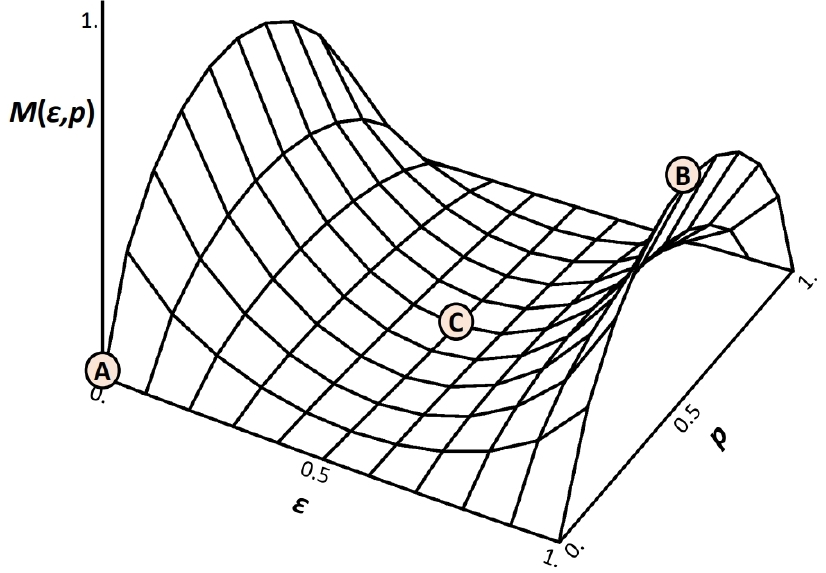
\includegraphics[width=0.4\textwidth]{entropy-plot}

    \end{figure}

    \begin{enumerate}

        \item At the point marked $A$, the error probability is $\epsilon = 0$. Why then is the channel mutual information minimal in this case: $M(\epsilon, p) = 0$?

        $p = 0$. Thus receiving a $0$ is certain and so conveys no information. We have $I(X; Y) = H(X) - H(X \mid Y) = 0 - 0 = 0$.

        \item At the point marked $B$, an error always occurs $(\epsilon = 1)$. Why then is the channel mutual information maximal in this case: $M(\epsilon, p) = 1$. At this point, the error probability is $1$.

        Error probability of $1$ means that on receiving symbol $\sigma$, we are guaranteed the original message was $1 - \sigma$. So on receiving a message we have no uncertainty about its value: i.e.\@
        $H(X \mid Y) = 0$. So we have $I(X; Y) = H(X) - H(X \mid Y) = H(X)$. Since $p = 0.5$, we have $H(X) = 1$ and so $I(X; Y) = 1$.

        \item At the point marked $C$, the input bit values are equiprobable $(p = 0.5)$, so the symbol source has maximal entropy. Why then is the channel mutual information in this case $M(\epsilon, p) = 0$.

        $H(Y \mid X) = 1$: knowing the output tells us nothing about the input! So, even though we have $H(X) = H(Y) = 1$, we have $I(X; Y) = H(Y) - H(Y \mid X) = 1 - 1 = 0$.

    \end{enumerate}

\end{enumerate}

\end{document}
